%Version 2.1 April 2023
% See section 11 of the User Manual for version history
%
%%%%%%%%%%%%%%%%%%%%%%%%%%%%%%%%%%%%%%%%%%%%%%%%%%%%%%%%%%%%%%%%%%%%%%
%%                                                                 %%
%% Please do not use \input{...} to include other tex files.       %%
%% Submit your LaTeX manuscript as one .tex document.              %%
%%                                                                 %%
%% All additional figures and files should be attached             %%
%% separately and not embedded in the \TeX\ document itself.       %%
%%                                                                 %%
%%%%%%%%%%%%%%%%%%%%%%%%%%%%%%%%%%%%%%%%%%%%%%%%%%%%%%%%%%%%%%%%%%%%%

\documentclass[sn-basic,pdflatex]{sn-jnl}

%%%% Standard Packages
%%<additional latex packages if required can be included here>

\usepackage{graphicx}%
\usepackage{multirow}%
\usepackage{amsmath,amssymb,amsfonts}%
\usepackage{amsthm}%
\usepackage{mathrsfs}%
\usepackage[title]{appendix}%
\usepackage{xcolor}%
\usepackage{textcomp}%
\usepackage{manyfoot}%
\usepackage{booktabs}%
\usepackage{algorithm}%
\usepackage{algorithmicx}%
\usepackage{algpseudocode}%
\usepackage{listings}%
%%%%

%%%%%=============================================================================%%%%
%%%%  Remarks: This template is provided to aid authors with the preparation
%%%%  of original research articles intended for submission to journals published
%%%%  by Springer Nature. The guidance has been prepared in partnership with
%%%%  production teams to conform to Springer Nature technical requirements.
%%%%  Editorial and presentation requirements differ among journal portfolios and
%%%%  research disciplines. You may find sections in this template are irrelevant
%%%%  to your work and are empowered to omit any such section if allowed by the
%%%%  journal you intend to submit to. The submission guidelines and policies
%%%%  of the journal take precedence. A detailed User Manual is available in the
%%%%  template package for technical guidance.
%%%%%=============================================================================%%%%

%% Per the spinger doc, new theorem styles can be included using built in style, 
%% but it seems the don't work so commented below
%\theoremstyle{thmstyleone}%
\newtheorem{theorem}{Theorem}%  meant for continuous numbers
%%\newtheorem{theorem}{Theorem}[section]% meant for sectionwise numbers
%% optional argument [theorem] produces theorem numbering sequence instead of independent numbers for Proposition
\newtheorem{proposition}[theorem]{Proposition}%
%%\newtheorem{proposition}{Proposition}% to get separate numbers for theorem and proposition etc.

%% \theoremstyle{thmstyletwo}%
\theoremstyle{remark}
\newtheorem{example}{Example}%
\newtheorem{remark}{Remark}%

%% \theoremstyle{thmstylethree}%
\theoremstyle{definition}
\newtheorem{definition}{Definition}%



\raggedbottom




% tightlist command for lists without linebreak
\providecommand{\tightlist}{%
  \setlength{\itemsep}{0pt}\setlength{\parskip}{0pt}}

% From pandoc table feature
\usepackage{longtable,booktabs,array}
\usepackage{calc} % for calculating minipage widths
% Correct order of tables after \paragraph or \subparagraph
\usepackage{etoolbox}
\makeatletter
\patchcmd\longtable{\par}{\if@noskipsec\mbox{}\fi\par}{}{}
\makeatother
% Allow footnotes in longtable head/foot
\IfFileExists{footnotehyper.sty}{\usepackage{footnotehyper}}{\usepackage{footnote}}
\makesavenoteenv{longtable}




\begin{document}


\title[Article Title runing]{Estudo Comparativo de Planos Amostrais
Complexos na Estimação da Média de Notas Escolares}

%%=============================================================%%
%% Prefix	-> \pfx{Dr}
%% GivenName	-> \fnm{Joergen W.}
%% Particle	-> \spfx{van der} -> surname prefix
%% FamilyName	-> \sur{Ploeg}
%% Suffix	-> \sfx{IV}
%% NatureName	-> \tanm{Poet Laureate} -> Title after name
%% Degrees	-> \dgr{MSc, PhD}
%% \author*[1,2]{\pfx{Dr} \fnm{Joergen W.} \spfx{van der} \sur{Ploeg} \sfx{IV} \tanm{Poet Laureate}
%%                 \dgr{MSc, PhD}}\email{iauthor@gmail.com}
%%=============================================================%%

\author[1]{\fnm{Pedro} \spfx{Henrique Corrêa de} \sur{Almeida} }

\author[1]{\fnm{Gustavo} \spfx{Almeida} \sur{Silva} }



  \affil*[1]{\orgdiv{Dep. Estatística, Instituto de Ciências
Exatas}, \orgname{Universidade Federal de Juiz de
Fora}, \orgaddress{\city{Juiz de Fora}, \country{MG}, \state{Brasil}}}

\abstract{Buscando comparar o desempenho de diferentes planos amostrais
em um mesmo conjunto de dados, este trabalho utiliza o método de
simulação Monte Carlo para geração de amostras. Os dados simulados são
então analisados usando técnicas estatísticas apropriadas para avaliar o
viés, erros padrão e outras medidas relevantes para cada plano amostral.
Os resultados desta pesquisa contribuem para a compreensão dos pontos
fortes e limitações das pesquisas estratificadas e em múltiplos
conglomerados. O estudo destaca a importância de considerar desenhos de
amostragem complexos e suas métricas associadas para obter estimativas
confiáveis e robustas. Os resultados das simulações fornecem insights
valiosos sobre a adequação e o desempenho dos métodos de amostragem
conglomerada em diferentes estágios. Espera-se que este estudo contribua
para a compreensão das complexidades da amostragem em pesquisas com
estrutura hierárquica e auxilie pesquisadores na escolha do método de
amostragem mais apropriado para suas necessidades.}

\keywords{Amostragem, Plano Amostral Complexo, Amostragem
Estratificada, Amostragem por Conglomerado, Simulação Monte Carlo}



\maketitle

\newpage

.

\hypertarget{introduuxe7uxe3o}{%
\section{Introdução}\label{introduuxe7uxe3o}}

A amostragem desempenha um papel fundamental na estatística, permitindo
aos pesquisadores obterem informações sobre uma população a partir de
uma amostra representativa. Através de métodos estatísticos robustos, é
possível extrapolar conclusões precisas e confiáveis sobre a população
em geral. No entanto, a amostragem muitas vezes enfrenta desafios
práticos, como a seleção adequada das unidades amostrais e a
consideração de complexidades inerentes a certos planos de amostragem.

De forma geral, é amplamente reconhecido na teoria da amostragem que,
embora o esquema de amostragem aleatória simples (AAS) seja teoricamente
simples, na prática, é pouco utilizado devido às restrições
orçamentárias e à busca por métodos probabilísticos que forneçam
informações mais precisas. Além disso, é comum encontrar dificuldades na
obtenção de cadastros adequados para o AAS, bem como lidar com situações
de não resposta, o que requer considerar observações com pesos desiguais
\citep{skinner2005design}. A especificação inadequada na análise do
plano amostral selecionado também pode resultar em estimativas
enviesadas, destacando a importância de estudar metodologias que levem
em conta o esquema de amostragem adotado.

A simulação de Monte Carlo é uma técnica estatística que envolve a
geração de múltiplas amostras aleatórias com base em modelos
probabilísticos. É amplamente utilizada para avaliar incertezas, estimar
parâmetros e estudar o desempenho de métodos estatísticos em uma
variedade de áreas \citep{kroese2012monte}.

Nesse contexto, o trabalho tem como objetivo explorar a interseção entre
a amostragem e a simulação computacional via método Monte Carlo,
destacando como essa abordagem combinada pode contribuir para aprimorar
a qualidade das inferências estatísticas. Serão apresentados conceitos
fundamentais da amostragem, incluindo diferentes métodos de seleção
amostral e as respectivas propriedades, e, em seguida, será discutido
como a simulação computacional pode ser aplicada para investigar essas
técnicas em contextos específicos.

Ao integrar a simulação computacional à amostragem estatística, os
pesquisadores podem explorar virtualmente uma ampla gama de cenários de
amostragem, considerando diferentes planos amostrais, tamanhos de
amostra e distribuições populacionais. Além disso, a simulação permite a
avaliação de métricas de desempenho, como viés e erro padrão, fornecendo
insights valiosos sobre a precisão e a eficiência dos métodos de
amostragem em diferentes contextos.

\hypertarget{metodologia}{%
\section{Metodologia}\label{metodologia}}

O objetivo deste trabalho é comparar diferentes planos de amostragem em
estágios complexos, como a amostragem estratificada e a amostragem
conglomerada. Para realizar essa comparação, foi conduzido um estudo de
simulação via método de Monte Carlo. O estudo tem como propósito
investigar e avaliar o desempenho desses diferentes planos amostrais em
termos de eficiência, precisão e viés. Através da simulação, é possível
criar cenários controlados que permitem analisar o impacto de cada plano
amostral em diferentes características da população. Com base nos
resultados obtidos na simulação, foi possível identificar quais planos
de amostragem são mais adequados para determinados contextos e auxiliar
na tomada de decisões estatísticas mais embasadas.

Para isso, foi utilizado o conjunto de dados: \textbf{Alunos.txt}, que
se trata de dados sobre notas de alunos em um determinado teste de
português. Os dados são populacionais. Assim, diferentes métodos de
amostragem complexa foram avaliados utilizando esse conjunto de dados.

O conjunto de dados possui 6 variáveis, são elas:

\begin{longtable}[]{@{}
  >{\raggedright\arraybackslash}p{(\columnwidth - 2\tabcolsep) * \real{0.32}}
  >{\raggedright\arraybackslash}p{(\columnwidth - 2\tabcolsep) * \real{0.68}}@{}}
\toprule
\begin{minipage}[b]{\linewidth}\raggedright
Variável
\end{minipage} & \begin{minipage}[b]{\linewidth}\raggedright
Descrição
\end{minipage} \\
\midrule
\endhead
Aluno & ID do aluno \\
Rede & Rede de ensino \\
Escola & ID da escola \\
Turma & ID da turma \\
Port & Nota no teste de portugues de cada aluno, é tambem a variável de
interesse desse trabalho \\
\bottomrule
\end{longtable}

Os metodos estudados foram:

\begin{itemize}
\item
  Amostragem Estratificada

  \begin{itemize}
  \tightlist
  \item
    Foram testados estratificação por Rede e estratificação por Escola
  \end{itemize}
\item
  Amostragem Conglomerada

  \begin{itemize}
  \item
    1 estágio por Escolas
  \item
    1 estágio por Turmas
  \item
    2 estágios: UPA-Escolas, USA-Turmas
  \item
    3 estágios: UPA-Escolas, USA-Turmas, UTA-Alunos
  \end{itemize}
\item
  Amostragem Conglomerada com PPT Poisson

  \begin{itemize}
  \tightlist
  \item
    1 estágio por Escolas, tamanho via número de turmas
  \item
    1 estágio por Escolas, tamanho via número de alunos
  \end{itemize}
\end{itemize}

\hypertarget{estudo-de-simulauxe7uxe3o}{%
\section{Estudo de Simulação}\label{estudo-de-simulauxe7uxe3o}}

Considerou-se como variavel de interesse a média da variavel Port com
transformação logaritmo natural, ou seja, a variavel estimada via
diferentes metodos de amostragem complexa foi: \(ln({Port})\)

Para a cada plano amostral, foram replicadas 1000 vezes amostras de
tamanho 500 e 750, para cada replicação foram calculadas as estimativas
pontuais e seu o erro padrão

Para avaliar o desempenho de cada plano amostral. foram consideradas
metricas como \textbf{Víes, Erro-padrão, Erro Quadrático Médio e a
Proporção de captação do valor paramétrico no intervalo de confiança de
\(95\%\) da estimativa}.

O verdadeiro valor da variável estimada é de:

\[
\frac{\sum_{i=1}^n{ln(Port_i)}}{n} = 6.218181
\]

O conhecimento de tal valor é importantíssimo para o calculo do viés e
consequente a decisão sobre o plano maostral mais adequado para o
problema.

Construi-se o seguinte diagrama para facilitar passo a passo aplicado
durante as seguintes etapas:

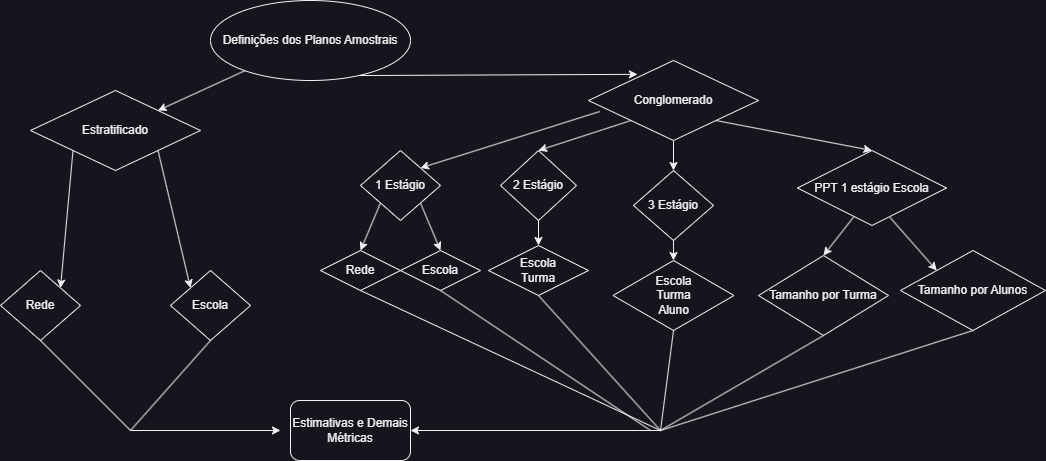
\includegraphics[width=\textwidth,height=0.3\textheight]{D:/UFJF_materias/Amostragem2/survey_articles/Untitled/figs/schema_simulation.png}

\hypertarget{amostragem-estratificada}{%
\subsection{Amostragem Estratificada}\label{amostragem-estratificada}}

A amostragem estratificada é uma técnica valiosa que permite uma seleção
mais precisa e representativa da amostra, considerando as
heterogeneidades presentes na população. Ao estratificar a população em
subgrupos e selecionar uma amostra de cada estrato, é possível obter
estimativas mais confiáveis e insights mais detalhados sobre os
diferentes grupos presentes na população de interesse.

O estimador não viciado do parâmetro de média é dado por:

\[\bar{y_h} = \sum_{i=1}^{n_h}\frac{y_{hi}}{n_h}\]

Enquanto o estimador da variância do estimador de média é dado por:

\[\hat V_{AES}(\bar y_{AES}) = \sum_{h=1}^{H}W_h^2(\frac{1}{n_h}-\frac{1}{N_h})s_h^2\]

Nesse contexto, trabalhou-se com duas divisões de estratos: Rede e
Escola.

Primeiramente foi realizada 1000 replicações com um tamanho amostral
igual a 500, após isso realizou-se novamente 1000 replicações com 750.

Foram consideradas 3 tipos de alocação amostral

\begin{itemize}
\item
  Uniforme
\item
  Proporcional ao Tamanho
\item
  Ótima de Neyman
\end{itemize}

\hypertarget{estratificada-por-rede}{%
\subsubsection{Estratificada por Rede}\label{estratificada-por-rede}}

Após aplicar as 1000 replicações utilizando o método de Monte Carlo,
obteu-se as seguintes estimativas

\hypertarget{n-500}{%
\paragraph{n = 500}\label{n-500}}

\begin{longtable}[]{@{}llllll@{}}
\toprule
Alocação & \(\hat{\theta}\) & \(\hat{EP(\theta)}\) &
\(IC(95\%)\subset \theta\) & Viés & EQM \\
\midrule
\endhead
Uniforme & 6.218338 & 0.0104576 & 0.966 & 0.0001568 & 0.0001094 \\
Proporcional & 6.218293 & 0.0090885 & 0.951 & 0.0001121 & 0.0000826 \\
Neyman & 6.218179 & 0.0090841 & 0.964 & -0.0000020 & 0.0000825 \\
\bottomrule
\end{longtable}

Vemos um ótimo desempenho dos 3 tipos de alocação, onde todos
apresentaram um EQM extremamente baixo. O intervalo de confiança
considerado foi de \(95%
\), assim vemos que o metodo de alocação Proporcional foi aquele que
mais se aproximou desse valor. Os demais metodos apresentaram taxa de
rejeição inferior ao nivel de significancia definida.

\hypertarget{n-750}{%
\paragraph{n = 750}\label{n-750}}

\begin{longtable}[]{@{}llllll@{}}
\toprule
Alocação & Estimativas & ErroPadrão & \(IC(95\%)\subset \theta\) & Viés
& EQM \\
\midrule
\endhead
Uniforme & 6.217622 & 0.0085606 & 0.968 & -0.0005597 & 7.36e-05 \\
Proporcional & 6.218224 & 0.0074278 & 0.960 & 0.0000427 & 5.52e-05 \\
Neyman & 6.217922 & 0.0074324 & 0.966 & -0.0002592 & 5.53e-05 \\
\bottomrule
\end{longtable}

Com base nos resultados obtidos a partir do estudo de simulação, pode-se
verificar que os intervalos de confiança de 95\% conteram o valor real,
aproximadamente, 95\% das vezes, como era o esperado. Além disso, viu-se
que, a alocação Uniforme apresentou o maior erro quadrático médio entre
as 3 alocações, por outro lado as alocações Proporcional e Ótima de
Neyman tiveram resultados semelhantes.

Além disso, podemos verificar, que o erro padrão e o erro quadrático
médio apresentou diminuição ao aumentar o tamanho amostral. No entanto,
não houve uma melhora significativa em relação ao viés.

\hypertarget{estratificada-por-escola}{%
\subsubsection{Estratificada por
Escola}\label{estratificada-por-escola}}

\begin{longtable}[]{@{}llllll@{}}
\toprule
Alocação & Estimativas & ErroPadrão & \(IC(95\%)\subset \theta\) & Viés
& EQM \\
\midrule
\endhead
Uniforme & 6.218014 & 0.0094822 & 0.981 & -0.0001673 & 8.99e-05 \\
Proporcional & 6.217734 & 0.0084041 & 0.983 & -0.0004475 & 7.08e-05 \\
Neyman & 6.217978 & 0.0086743 & 0.986 & -0.0002035 & 7.53e-05 \\
\bottomrule
\end{longtable}

Os 3 metodos apresentaram um erro quadrático médio baixo, porém o
intervalo de confiança não obteve desempenho desejado. Definido um nivel
de confiança de \(5\%\), viu-se que os três métodos apresentaram um
nível de rejeição menor que o esperado.

\begin{longtable}[]{@{}llllll@{}}
\toprule
Alocação & Estimativas & ErroPadrão & \(IC(95\%)\subset \theta\) & Viés
& EQM \\
\midrule
\endhead
Uniforme & 6.218394 & 0.0081765 & 0.982 & 0.0002125 & 6.69e-05 \\
Proporcional & 6.218155 & 0.0070644 & 0.991 & -0.0000268 & 4.99e-05 \\
Neyman & 6.218010 & 0.0072053 & 0.984 & -0.0001719 & 5.19e-05 \\
\bottomrule
\end{longtable}

Apesar do aumento do tamanho amostral, não observou-se uma diminuição do
\textbf{EQM}, além disso o 3 métodos apresentaram alta de taxa de não
rejição em seus intervalos de confiança, ou seja, um rejeição bem menor
que \(5\%\)

\hypertarget{amostragem-conglomerada}{%
\subsection{Amostragem Conglomerada}\label{amostragem-conglomerada}}

A principal motivação por trás da amostragem conglomerada é simplificar
o processo de amostragem quando a população é muito grande ou
geograficamente dispersa. Em vez de lidar com cada elemento
individualmente, os conglomerados podem ser selecionados de forma mais
eficiente, reduzindo os custos e o tempo necessários para a coleta de
dados. Esse método apresenta custos de operações menores quando
comparados a outro métodos amostrais

O estimador não viciado do parâmetro de média por conglomerado é dado
por:

\[\bar{y_N} = \frac{\hat{Y}}{M_0}\]

Enquanto o estimador da variância do estimador natural é dado por:

\[\hat V_{ACS}(\bar y_{N}) = \frac{1}{\bar M^2}\frac{1-f}{n}s_e^2\]

\hypertarget{tempo-de-execuuxe7uxe3o-computacional}{%
\section{Tempo de execução
computacional}\label{tempo-de-execuuxe7uxe3o-computacional}}

Durante a construção do trabalho, certos planos amostrais apresentaram
um desempenho ligeiramente melhor que outros, porém tal melhoria um
tempo de execução computacional razoável.

Uma métrica importantíssima que as métricas estatísticas não captam é
aquela de tempo de execução computacional, tal métrica pode indicar qual
plano amostral é superior quando as métricas estatísticas se mostrarem
próximas

Assim, este tópico busca comparar os tempos de execução computacional
dos métodos já estudados

Tempo de execução para calculos de estimativas a partir de uma amostra
já definida é ínfimo quando comparado ao tempo de execução de funções de
calculado de alocação e seleção amostral, assim apenas as funções de
alocação e seleção amostral foram utilizadas para a estimativa do tempo
gasto. \footnote{Setup: Intel i5-11400; 8gb à 2666mhz}

\begin{itemize}
\tightlist
\item
  Amostragem Estratificada
\end{itemize}

\begin{longtable}[]{@{}llllll@{}}
\toprule
Alocação & Média por Replicação & Total & & & \\
\midrule
\endhead
Uniforme & 6.218394 & 0.0081765 & 0.982 & 0.0002125 & 6.69e-05 \\
Proporcional & 6.218155 & 0.0070644 & 0.991 & -0.0000268 & 4.99e-05 \\
Neyman & 6.218010 & 0.0072053 & 0.984 & -0.0001719 & 5.19e-05 \\
\bottomrule
\end{longtable}

\hypertarget{conclusuxe3o}{%
\section{Conclusão}\label{conclusuxe3o}}

\citet{pfeffermann1996use}, \citet{kleijnen1995verification}

\bibliography{bibliography.bib}


\end{document}
